\documentclass[a4paper]{jreport}	% 日本語の場合

\usepackage{masterThesisJa}
\usepackage{graphicx}
\usepackage{float}
\setcounter{tocdepth}{3}
\setcounter{page}{-1}
\usepackage{url} 




% 【必須】主題:\maintatile{日本語}{英語}
\maintitle{Elixirを基く画像処理フォールトトレラントパイプラインの構築と評価}

% 【任意】副題:\subtitle{日本語}{英語}
% 副題が不要な場合は次の行をコメントアウトしてください
\subtitle{Construction and evaluation of image processing fault-tolerant pipeline based on elixir}

% 【必須】発表年月:\publish{年}{月}
\publish{2024}{03}



% 【必須】学生情報:\student{学籍番号}{氏名(日本語:氏名の間は1文字空ける)}{氏名(英語:Twins登録の表記)}
\student{20XX21XXX}{ヨウ サイケイ}

% 【必須】日本語の概要:\jabst{概要}

%\jabst{ この文書は、北九州市立大学}

% 【任意】英語の概要:\eabst{Abstract}
% 英語の概要が不要な場合は\eabst{}をすべてコメントアウトしてください
%\eabst{\\ 英語をつけてもよい}

% 【必須】研究指導教員(氏名の間は1文字空ける):\advisors{主研究指導教員}{副研究指導教員}
%\advisors{山崎 進}


% 以下,本文を出力
\begin{document}

\makecover

\addtolength{\textheight}{-5mm}	% 本文の下限を5mm上昇
\setlength{\footskip}{15mm}	% フッタの高さを15mmに設定
\fontsize{11pt}{15pt}\selectfont

% 目次・表目次を出力
\pagebreak\setcounter{page}{1}
\pagenumbering{roman} % I, II, III, IV 
\pagestyle{plain}
\tableofcontents
%\listoffigures
%\listoftables

% 本文
\parindent=1zw	% インデントを1文字分に設定
\pagebreak\setcounter{page}{1}
\pagenumbering{arabic} % 1,2,3
\pagestyle{plain}

% 章:\chapter{}
% 節:\section{}
% 項:\subsection{}

\chapter{はじめに}
\section{背景}
近年,画像処理技術は現代では非常に普及しており,私たちの日常生活のさまざまな局面で広く活用されている.たとえば,医療画像,衛星画像分析,物体認識,スペクトル分析などである.また,画像処理の精度を向上させるために,機械学習を使う画像処理の大規模化・複雑化が顕著に進んでいる\cite{A}.
\\ このような画像処理では,大量のデータを高速処理することが求められるため,高速化を実現する1つの手段としてマルチコア等を使った並列処理が重要となる.ただし,画像処理のシステムにおいて,マルチコアプロセッサシステム上でコードを実行しても,自動的にコードが効率化されるわけではない.また,並行・並列プログラミングにおいて,デッドロックや性能低下の問題がある\cite{B}.
\\ 画像処理のソフトウェア全体で最適な並列化を実現するため,山崎らがElixirに着目し,画像処理のデファクトスタンダードであるPythonと比べてElixirの潜在的優位性を示した\cite{C}.
\\ 画像処理にElixirをより効率的に使うために,NxとEvisionが開発された.Nxは高速的に行列変換に対処できる.Evisionは画像処理に対処できる.
\\ しかし,NxとEvisionを使って,巨大な画像を処理すると,メモリ不足などによる異常終了になることがある.特にEvisionとNxのアクセラレータであるEXLAがNIF関数を使用しており,NIF関数が異常終了すると,Erlang VM 全体が異常終了になる可能性がある.
\\ このように多様かつ複雑なアプリケーションは画像処理システムの異常終了により,極端な場合,人命や巨額の金銭が危険にさらされる可能性がある.
\\ したがって,このような画像処理システムの構築において耐障害性はかなり重要な部分である.
\\ 画像処理において耐障害性の高いパイプラインを構築するために,山崎進は2022年のElixirConfで巨大な画像に対する堅牢な分散並列処理について講演し,HtPipeを提案した\cite{E}.HtPipeはNIF関数が異常終了することで,Erlang VM全体が異常終了するのは回避できるが,並列処理で関数の作成と呼び出しにはBroadwayを使用する方が簡潔で効率的である.また,Broadwayではデータの生成部分と処理部分が分離されており,一時的に一部の機能が失われたとしても,データの流れは整然と処理される.
\\ したがって,そのようなパイプラインには,まだ改善すべき部分が存在していると考えられる.このような背景から,我々は,Broadwayのデータ取り込みとデータ処理機能を画像処理パイプラインとして活用することに着目する.

\section{目的}
この研究の目標は,画像処理を行うBroadwayパイプラインを構築し,その中でNodeを用いることで,耐障害性を向上させたパイプラインの開発と評価を行うことである.
\section{アプローチ}
\subsection{研究手段}
本研究では,耐障害性を向上させたパイプラインの開発するための足掛かりとして,Elixirのライブラリ関数のBroadwayをHtPipeと機能等価なパイプラインとして設計することに取り組む.
\\ 一つは,Broadway自体のSupervisorを使って,Broadway内の個々のプロセスを監視し,巨大な画像を処理すると,メモリ不足などによる異常終了が発生した場合に再起動する.これによって,異常終了になることを避ける.
\\ もう一つは,Nodeの動作における親と子のノード間のメッセージ通信を介して,クラッシュの原因となるNIF関数は子ノードで呼び出されて,このようにして,子のノードがクラッシュした後でも,親ノードが影響を受けない.これによって,NIFが異常終了しても,起動元のErlang VMに波及することはないである.
\subsection{評価手法}
まず,実装を行ったBroadwayパイプラインについて安全性・回復速度の 2 つの観点から性能を評価する.

安全性の有効性を証明する為に,二重システム制御実験評価にはFault-Injection (以下,FI と略す)を使用して,子プロセスをシャットダウンする関数1とabortを伴う NIF 関数2を作成する.

さらに,作成した関数 1 と関数 2 をそれぞれパイプラインがインストールされている環境とインストールされていない環境で呼び出す.Broadwayパイプラインの回復機能に基づくパイプラインに関するフォールトトレランスの効果評価する.

最後, Benchee を使用して, 実際にメモリ不足などによる異常終了が発生した場合, 回復速度をテストを行う.
\section{論文の構成}
本論文の構成は,以下のとおりである.2章に本手法を実装するうえで基となるBroadwayとNodeについて述べる.3章において,画像処理を行うBroadwayパイプラインの提案と実装方法について説明し,第4章で実装成果の評価結果を示す.第5章で本稿をまとめる.


\chapter{関連研究}
\section{Broadway}
Broadway は,Elixir チームによってデータパイプラインを作成および管理できるツールである.イベントと,メトリクス,自動応答,障害処理などの運用機能に重点を置いている\cite{D}.本章では,2.1.1 節で,Broadway の耐故障性能の基盤技術となるBroadwayのSupervisor動作について簡単に述べたうえで,2.1.2 節で Broadwayにおけるデータ処理パイプラインを作成するための構成要素GenServerについて述べる.
\subsection{BroadwayのSupervisor動作}
BroadwayのSupervisorは職場でスーパーバイザーが従業員のグループに対して責任を負うのと同じように,割り当てられたプロセスに対して責任を負う.下位プロセスも上司に報告する必要があり,上司はすべてがスムーズに実行されていることを確認する必要がある.これを実現するために,スーパーバイザには,他のプロセスを効果的に管理できる一連の機能が付属している. プロセスを開始および停止したり,システム内で予期しないエラーが発生した場合にはプロセスを再起動したりできる.これらは終了をトラップするように構成されているため,監視対象プロセスがエラーで終了すると,そのエラーは隔離され,それ以上伝播することはないである. 

Broadway の Supervisor 動作は,主に以下の部品により 構成されており,それぞれの関係を図 2.1 に表す.
\begin{figure}[H]
\vspace{11cm}
\begin{center}
\hspace{-13cm}
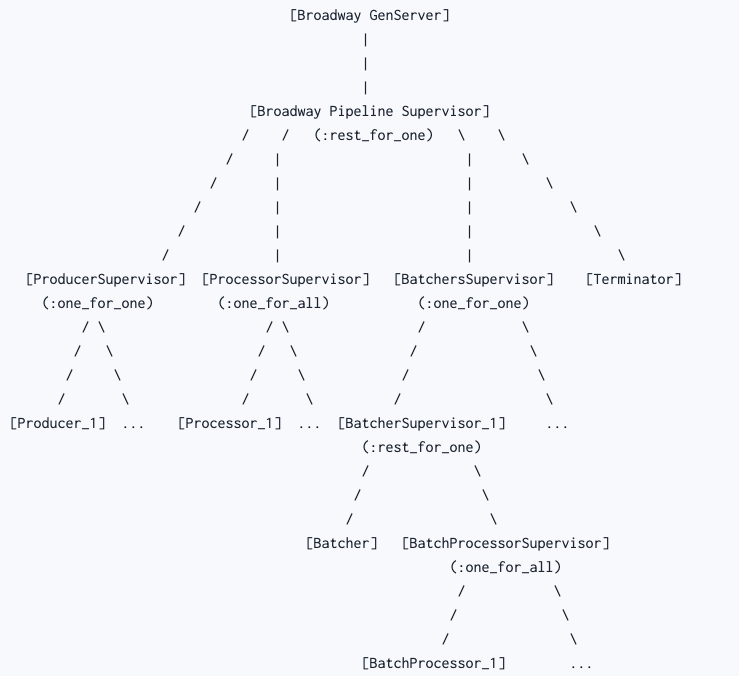
\includegraphics[scale=0.55]{ja/f2.png}
\end{center}
\caption{Broadwayの内部構造図}
\end{figure}
ツリーの最上部には,プロジェクト スーパーバイザーである Broadway Pipeline Supervisorがあり,\textbf{application.ex} ファイルで定義されている.

def start(\_type, \_args) do 

children = [

    \# Starts a worker by calling: Broadway.worker.start\_link(arg)
    
    
]

 \# See https://hexdocs.pm/elixir/Supervisor.html

 \# for other strategies and supported options

opts = [strategy: :one\_for\_one, name: Broadway.Supervisor] 

Supervisor.start\_link(children, opts)

end

Broadway Pipeline Supervisorは,Broadwayのさまざまなコンポーネントをすべて監視し,エラーが発生した場合は再起動する機能を持っている.Broadway Pipeline Supervisorが監視するプロセスとその目的を以下に示す.

\textbf{• ProducerSupervisor}:データ プロデューサー プロセスの監視を担当する. この監視ツリーには,問題が発生している特定のデータ プロデューサーのみを再起動する必要があるため,:one\_for\_one の戦略が採用されている.すべてが問題なければ,他のすべてのプロデューサーは実行を続けることができる.

\textbf{• ProcessSupervisor}:プロデューサーからのデータを消費するワーカー プロセスを監視する責任がある.この監視ツリーには,:one\_for\_all の戦略がある.これが :one\_for\_one ではない理由は作成する処理コールバック関数がステートレスである必要があり,発生したエラーはプロセスをクラッシュさせることなく処理できるためである.エラーが発生してプロセスがクラッシュした場合は,Broadwayに関連する内部簿記の一部に問題が発生している可能性があ,すべてのコンシューマーを再起動する必要がある.

\textbf{• BatchersSupervisor}: バッチを動的に監視するために使用できる.この監視ツリーには,:one\_for\_all の戦略がある.これが :one\_for\_one ではない理由はProcessSupervisorと同じである.

\textbf{• Terminator: Broadway}パイプラインを適切に停止する責任がある.これは,すべてのコンシューマ プロセスに,終了後にプロデューサに再サブスクライブしてはならないことを通知する.また,すべてのプロデューサに対して,現在のイベントをすべてフラッシュし,後続のデータ要求を無視するように通知する.

Broadway Pipeline Supervisorには :rest\_for\_one という監視ポリシーがあることも重要である. その理由は,プロデューサー監視ツリーがクラッシュした場合,親Supervisorは後続のすべての監視ツリーを再起動し,パイプラインを動作中の新しい状態に復元できるためである.


これらすべてにより,Supervisorは耐故障性能の基盤技術となる.

\subsection{BroadwayのGenServer動作}
GenServer(generic serverの略) は,クライアントとサーバーの関係のサーバーを実装するための動作モジュールである.状態を保持したり,コードを非同期に実行したりするために使用されるだけではない.また,標準的なインターフェイス関数セットがあり,トレースおよびエラー報告の機能も含まれる\cite{M}.

GenServer モジュールは,GenServer の動作に必要ないくつかの関数のデフォルト実装を提供する.これらの関数はコールバックとして機能する.コールバックを実装するときは,次の 2 つのことを知っておく必要がある.

• コールバック関数が受け取る引数

• どのような戻り値がサポートされている

GenServer の動作に関する次のコールバック関数について説明する.

\textbf{• handle\_call/3}

handle\_call/3 は,クライアントから GenServer プロセスへの同期呼び出しを処理するために使用される.

\textbf{• handle\_cast/2}

handle\_cast/2 は,通常は他のプロセスまたはタイマーによってトリガーされる非同期イベントを処理するために使用される.

\textbf{• init/1}

init/1 は,GenServer プロセスの状態を初期化するために使用される必須のコールバック関数である. これはプロセスの開始時に呼び出され,通常はいくつかの初期化操作を実行するために使用され,プロセスの初期状態を含むタプルを返す.


これら 3 つのコールバック関数が一緒になって GenServer のコア動作を形成し,同期および非同期メッセージを処理できるようになり,Broadwayパイプラインが同時実行および並列実行を処理できるようになる.また,Broadwayパイプラインをカスタマイズできる.更にバックグラウンドでも実行される存続期間の長いプロセスを作成し,より優れた制御と柔軟性を提供する.


\section{Node}
Nodeは,ElixirがErlang言語から継承するライブラリ関数である\cite{H}.NodeによりElixirはErlangの強力な分散機能へアクセス可能である\cite{J}.

Nodeには,作成された各ノードは実行中の Erlang ランタイム システムとなる.ランタイム システムには,同時実行性,分散,フォールト トレランスのサポートが組み込まれている.

これによって,Elixirコンテキストでの配布は,言語の多くの機能がコードを変更せずにネットワーク上で動作することを意味する. 同時に,プロセスやメッセージ パッシングなどの基本的なプリミティブとプロセス リンクやモニターなどのより高度な概念も含まれる.

相互に接続する Erlang VM インスタンスは,Erlang ノードのクラスターと呼ばれる. Erlang ノードがクラスターに接続すると,その ID が他のすべてのノードに伝達され,Erlang ノードと他のすべてのノードの間に別のネットワーク接続が設定される.これは、いわゆる全結合メッシュになる.すべてのノードは他のすべてのノードに接続されているため,クラスター内の合計接続数は二次関数的に増加する.接続されたノードのセットのすべての接続の合計 c は \[ \sum_{c=1}^{n-1}c = \frac{n(n-1)}2\]で定義される.通常のポイントツーポイント トラフィックに加えて,Erlang ノードは各ノード接続上でティックと呼ばれるハートビート メッセージを送信し,リモートノードがまだ生きているかどうかを確認する.
\begin{figure}[H]
\vspace{4cm}
\begin{center}
\hspace{-5cm}
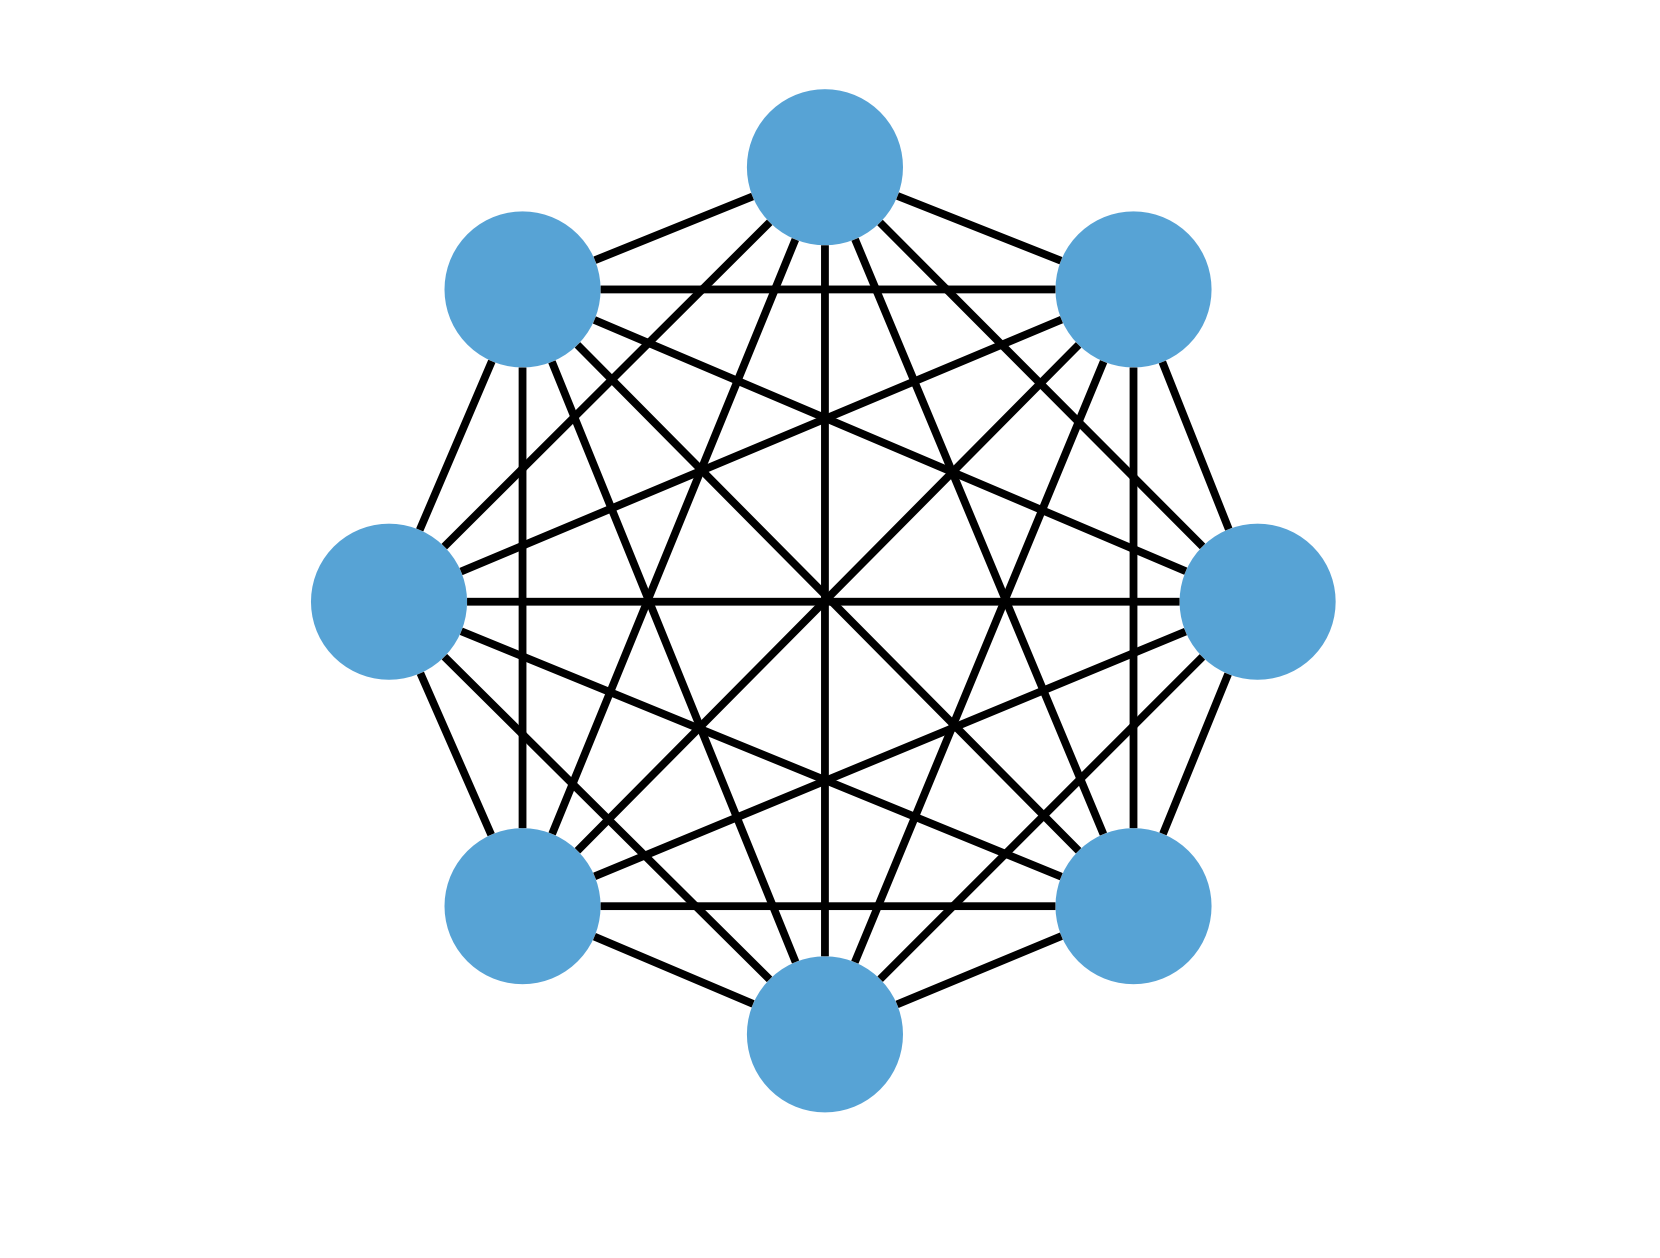
\includegraphics[scale=0.2]{ja/f1.png}
\end{center}
\caption{Node通信網}
\end{figure}

この一般的なアプローチにより,高い拡張性と耐障害性を備えたネットワーク ノードを構築できる. 分散 Erlang の元の設計は,プライベートの安全なネットワーク内で実行されることを目的としていた. したがって,デフォルトでは Erlang のノード間通信は暗号化されず \cite{I},共有秘密 (Cookie ) によってのみ保護される.異なるネットワーク内のノード間でメッセージを送信する時,同じ Cookie で起動されたノードのみが相互に正常に通信できる.

\section{SpawnCoElixir}
SpawnCoElixir は,山崎進によって書かれたElixirのライブラリ関数である.NodeとGenServerを使用して監視される協力的な Elixir ノードを起動,停止し,管理するためのコードを提供している\cite{N}.

本稿は,次の特徴を基づいてマルチノード フォールト トレランスに SpawnCoElixir を利用する.

\textbf{動的なノードの生成と管理:}

SpawnCoElixir は,動的なノードの生成と管理をできる.CoElixir ワーカーは,異なるノード上で動作できる.

\textbf{プロセスの監視と再起動:}

CoElixir ワーカープロセスは DynamicSupervisor で監視されており,プロセスがクラッシュした場合に再起動が行われる.これにより,ワーカーの耐障害性が向上できる.

\textbf{Elixir プロセスモデルの活用:}

SpawnCoElixir モジュールは Elixir プロセスモデルを活用しており,軽量かつ並列処理が容易である.これにより,大規模かつ複雑な分散システムの構築がしやすくなる.

\textbf{動的なコードの実行:}

SpawnCoElixir モジュールでは,動的にコードを指定して CoElixir ワーカーを生成できる.これにより,柔軟でカスタマイズ可能な実行環境を提供している。

\section{Benchee}
BencheeはElixir での簡単で優れた (マイクロ) ベンチマークのためのライブラリである. Benchee を使用すると, さまざまなコード部分のパフォーマンスを一目で比較できる. また, 関数だけに依存する多用途性と拡張性も備えている\cite{O}. 

実際のコード実行環境に近づけるために,Benchee は,最初のウォームアップ後に各関数を一定時間実行し, 実行時間と必要に応じてメモリ消費量を測定する. 次に,平均,標準偏差などのさまざまな統計値が表示される.

次の統計データ指標を説明する.

\textbf{average :} 平均実行時間/メモリ使用量である.

\textbf{ips :} 1 秒あたりの反復数,別名,指定された関数を 1 秒以内に実行できる頻度である.

\textbf{deviation :} 標準偏差である.

\textbf{median :} すべての測定値を並べ替えたときの中央の値である. 

\textbf{99 \% :} 最悪の場合のパフォーマンスである.

Benchee を使用すると,信頼性が高く,再現性があり,分析が簡単なパフォーマンス テストを作成できる. そして, Benchee を通じて取得されたデータは, Elixir コードのパフォーマンスを客観的に測定および比較するために使用できる.
\chapter{提案手法}
\section{提案手法の概要}
今回提案する一つ手法は,Elixir言語で画像処理に Broadwayのフォールトトレランスと並列処理を適用することを目指すというものである.Broadway は,スケーラブルなデータストリーム処理システムを構築するための Elixir のライブラリである.この提案は,特に画像の読み取り,画像の分割,保存操作などの画像バッチ処理にブロードウェイを使用することを目的としている. 

既存手法からの変更点は,画像処理にBroadwayを使用すると,並列処理プログラムがより簡潔に記述され,画像の流れがより明確になり得る.また,Broadway パイプラインで画像タスクを処理するときに監視および回復メカニズムにより,システムの耐障害性が向上し,プロセッサのクラッシュによる画像処理の中断が軽減される.

も一つ手法は,Elixirのライブラリ関数であるSpawnCoElixirの動作における親と子のノード間のメッセージ通信を介して,クラッシュの原因となる NIF 関数は子ノードで呼び出されて,このようにして,子のノードがクラッシュした後でも,親ノードが影響を受けない.これによって,NIF が異常終了しても,起動元の Erlang VM に波及することはないである.

%図3に既存手法 (C 言語を利用) と提案手法 (作成したBroadwayパイプラインを利用) の実行フローの比較図を示す.
\section{実装例}
以下で画像処理やマルチノード耐障害におけるBroadwayパイプラインについて述べる.
\subsection{パイプラインの基本構成}
パイプラインの基本構成:

def start\_link(\_opts) do

    Broadway.start\_link(\_ \_MODULE\_ \_,
    
      name: \_ \_MODULE\_\_,
      
      producer: [
      
        module: \{Counter, 1\},
        
        transformer: \{\_ \_MODULE\_ \_, :transform, [ ]\},
        
        concurrency: 1
        
       ],
       
      processors: [
      
        default: [concurrency: 4]
        
      ],
      
        batchers: [
        
        sqs: [concurrency: 2, batch\_size: 10],
        
        s3: [concurrency: 1, batch\_size: 10]
        
      ]
      
    )
    
end

このコードは,ElixirのBroadwayフレームワークを使用してパイプラインを開始するための関数である.以下に、このコードの主な機能と構造を説明する.

\textbf{Broadway.start\_link/2 }関数: これはBroadwayパイプラインを起動するための関数である.

\textbf{name: \_\_MODULE\_\_}: Broadwayパイプラインに名前を付けている.

\textbf{producer}: パイプラインの最初のステージであるプロデューサモジュールに関する設定である.

\textbf{transformer: \{\_\_MODULE\_\_, :transform, [ ]\}}: トランスフォーマモジュールに関する設定である.

\textbf{concurrency: 1, concurrency: 4}: パイプライン内の各ステージの並列処理の設定である.

\textbf{processors}: パイプライン内のプロセッサモジュールに関する設定である.

\textbf{batchers}: パイプライン内のバッチャモジュールに関する設定である.

この関数を呼び出すことで,Broadwayパイプラインが設定され,各ステージが連携してデータ処理が行われる.
\subsection{画像処理におけるパイプラインの実装}

\textbf{画像の読み取り:}

def init(\_a) do

    img1 = 
      "https://upload.wikimedia.org/wikipedia/en/7/7d/Lenna\_\%28test\_image\%29.png"
      
  |> HTTPoison.get!()
  
  |> then(\&(\&1.body))
  
  |> Evision.imdecode(Evision.Constant.cv\_IMREAD\_COLOR()) 
  
  \{:producer, img1\}
end

このinit/1関数はBroadwayパイプラインの初期化ステップを定義している.以下はこの関数の主な機能と構造を説明する.

\textbf{img1}の定義: この部分ではウェブ上の画像をURLからダウンロードして,それをElixirで扱える形式に変換している.

\textbf{HTTPoison.get!/1:} HTTPoisonライブラリを使用して指定されたURLから画像を取得する.

\textbf{then/2}: then/2は前のステップの結果を取り,関数を適用する.

\textbf{Evision.imdecode/2}: 画像のバイナリデータをEvisionライブラリを使用してデコードする.

\textbf{{:producer, img1}}: パイプラインの初期化の最後に,{:producer, img1}というタプルを返す.

この\textbf{init/1}関数は,Broadwayパイプラインが始まる際に一度だけ呼び出され,初期化のためのデータが設定される.

\textbf{閾値を指定して画像の二値化}:

\{threshold, mono\_img\} =

  src\_file

  |> Evision.imread(flags:
  
  Evision.Constant.cv\_IMREAD\_GRAYSCALE())
  
  |> Evision.threshold(127, 255, 
  
  Evision.Constant.cv\_THRESH\_BINARY())

このコードはEvisionライブラリを使用して画像のしきい値処理を行っている.以下はこのコードの主な機能と各部分の説明である.

\textbf{Evision.imread/1}: src\_fileで指定されたファイルをEvisionライブラリを使用して読み込む.

\textbf{Evision.Constant.cv\_IMREAD\_GRAYSCALE/1}:画像をグレースケールで読み込む.

\textbf{Evision.threshold/3}: 読み込まれたグレースケール画像に対して,しきい値処理を行う.127が閾値の下限で,255が閾値の上限である.

このコードは,指定された画像ファイルを読み込んでグレースケールに変換し,さらにしきい値処理を行っている.

\textbf{画像の分割}:

def handle\_demand(demand, img1) when demand > 0 do   

    src\_file = "Lenna.png"
    
    Evision.imwrite(src\_file, img1)
    
    div\_size = 256
    
    dst\_file\_ext = Path.extname(src\_file)
    
    dst\_file\_basename = Path.basename(src\_file, dst\_file\_ext)
    
    dst\_files =
    
      Stream.unfold(0, fn counter -> {counter, demand - 9} end)
      
      |> Stream.map(\&"\#{dst\_file\_basename}\_\#\{\&1\}\#\{dst\_file\_ext\}")
    
    div\_img =
    
    mono\_img
    
    |> Evision.Mat.to\_nx()
    
    |> Nx.to\_batched(div\_size)
    
    |> Enum.map(\&Evision.Mat.from\_nx\_2d(\&1))
    
    z\_img = 
    
    Enum.zip(div\_img, dst\_files)
    
    |> Enum.to\_list()
    
    \{:noreply, z\_img, dst\_files\}
  
end

この\textbf{handle\_demand/2}関数は,ElixirのGenStageのハンドラ関数である.以下はこの関数の主な機能と各部分の説明である.

\textbf{Evision.imwrite/2}: この関数を使用して img1(しきい値処理された画像)を "Lenna.png" に保存する.

\textbf{div\_size}: 画像を分割する際のサイズです.256として設定されている.

\textbf{dst\_files}: 各数字を "Lenna\_数字.png" のような形式のファイル名に変換する.これにより、分割された画像を保存するためのファイル名リストが作成される.

\textbf{div\_img:} mono\_imgをNx形式に変換し,指定されたサイズでバッチ処理した後,それを元に画像データを再構築する.

\textbf{z\_img}: div\_imgと dst\_filesを組み合わせて,それぞれの分割画像と対応するファイル名をタプルで持つリストを生成する.

最終的には、:noreplyとともに生成されたデータ(z\_imgとdst\_files)が返される.このデータはGenStageの次のステップに渡される.

\textbf{コマンドラインに出力}:

  def handle\_message(:default, message, \_context) do
  
    message.data
    
    |> Enum.map(fn {img, dst\_file} -> Evision.imwrite(dst\_file, img) end)
    
    |> IO.inspect
    
  end

この\textbf{handle\_message/3}関数はElixirのGenStageのハンドラ関数である.この関数は\textbf{:default}メッセージを処理する.以下はその機能の説明である.

\textbf{message.data}: メッセージのデータ部分を取得する.

\textbf{Enum.map/2}: メッセージのデータ部分(imgとdst\_fileのタプル)を取り出し,それぞれの組み合わせに対して\textbf{Evision.imwrite(dst\_file, img)} を実行する.これにより,各分割画像がそれに対応するファイル名で保存される.

\textbf{IO.inspect/1}: 最終的に生成されたリストを出力する.

この関数は \textbf{:default} メッセージを処理し,画像と対応するファイル名のリストを使って画像を保存する役割を果たしている.

\subsection{耐障害性を用いるパイプラインの実装}
SpawnCoElixirの構成オプションを定義する.

options = [

\{:code, "abort\_nif()"\},

\{:deps, []\},

\{:host\_name, "host"\},

\{:co\_elixir\_name, "co\_elixir"\}

]

\{:ok, \_\} = SpawnCoElixir.run(options)

\textbf{options}には 4 つの構成項目がある.Elixir コード,依存関係,ホスト ノード名プレフィックス,および CoElixir ノード名プレフィックスが含まれている.これらの構成項目は\textbf{SpawnCoElixir.run/1} 関数に渡され,Supervisorの監督で子ノードを起動し,渡された関数を実行する.

\subsection{abortをシミュレートするNIF関数の実装}

\#include <stdlib.h>

\#include <erl\_nif.h>

static ERL\_NIF\_TERM abort\_nif(ErlNifEnv *env, int argc, const ERL\_NIF\_TERM argv[])

\{

    abort();
    
\}

static ErlNifFunc nif\_funcs [] =

\{

    \{"abort\_nif", 0, abort\_nif\}
    
\};

ERL\_NIF\_INIT(Elixir.AbortNif, nif\_funcs, NULL, NULL, NULL, NULL)

このコードは,\textbf{Erlang NIF (Native Implemented Function)} と呼ばれる,C言語で書かれたErlangの拡張機能を作成する.abort\_nif関数は,C言語のabort()関数を呼び出している.これにより,Erlangプロセスがクラッシュし,Erlang VMが終了する.以下はコードの説明である.

\textbf{\#include <stdlib.h>}: 標準ライブラリのstdlib.hをインクルードしている.これは\textbf{abort()}関数が定義されているヘッダーファイルである.

\textbf{\#include <erl\_nif.h>}: Erlang NIFのためのヘッダーファイルをインクルードしている.

\textbf{static ERL\_NIF\_TERM abort\_nif}(ErlNifEnv *env, int argc, const ERL\_NIF\_TERM argv[]): abort\_nif関数が宣言されている.この関数は,Erlangから呼び出されるとabort()関数を実行し,プロセスをクラッシュさせる.引数としてenv(Erlangの実行環境),argc(引数の数),argv(引数のリスト)を取りる.

\textbf{static ErlNifFunc nif\_funcs [] }: 使用可能なNIF関数のリストが宣言されている.この例では,abort\_nif関数のエントリが含まれている.

\textbf{ERL\_NIF\_INIT(Elixir.AbortNif, nif\_funcs, NULL, NULL, NULL, NULL)}: NIFの初期化が行われる.これにより,NIFライブラリがErlang VMに登録され,Erlangコードから呼び出すことができる.

このNIFは,Erlangからの要求でabort()関数を呼び出してErlang VMを強制的にクラッシュさせるための関数である.

\chapter{評価実験}
本章では,提案するBroadwayパイプラインについて安全性・回復速度の 2 つの観点から性能を評価する.
まず4.1 節で,実験を行う際に用いた環境について述べる.そして4.2 節で提案手法の評価について述べ,4.3 節で障害の発生による耐故障処理の実験とBroadwayの性能について述べる.
\section{実験環境}
実験を行っ た環境は以下の通りである.

• OS : macOS Sonoma ver 14.1.1 

• CPU : Apple M1

• メモリ 16GB 

• Elixir 言語コンパイラ : Elixir 1.15.4

• Erlang 言語コンパイラ : Erlang/OTP 26 [erts-14.0.2]

• Broadway バージョン :  1.0.7

• Evision バージョン :  0.1.2

• Nx バージョン :  0.3.0

• SpawnCoElixir バージョン :  0.3.0

次の構成で実行されるベンチマーク スイート:

• warmup: 2 s

• time: 5 s

• memory time: 0 ns

• reduction time: 0 ns

• parallel: 1

• inputs: none specified

• Estimated total run time: 7 s

\section{評価手法}
提案するBroadwayパイプラインの評価実験は,安全性・回復速度の 2 つの観点から実施する.以下でそれぞれの項目について説明する.

\textbf{安全性:}

安全性の検証手法として,実際にメモリ不足などによる異常終了が発生した場合,再起動ができないかどうか実験を行う.

\textbf{回復速度:} 

Benchee を使用して,実際にメモリ不足などによる異常終了が発生した場合,回復速度をテストを行う.

実験は 3 つの部分に分かれている.

• 4.3.1 節ではパイプを使用して通常のタスクを処理する. パイプラインの可用性を確認する.

• 4.3.2 節では,FIを使用して,子プロセスをシャットダウンし,パイプラインで呼び出す関数1を作成する.タスクが異常終了したときの状況を実際にシミュレートする.プロセスの異常なシャットダウンに対する回復機能を確認してから,回復速度をテストを行う.

• 4.3.3 節では,FIを使用して,abortを伴う NIF 関数を作成し,パイプラインで呼び出す.NIF 関数の使用時に発生するabortをシミュレートする.NIF関数がabortされた後,起動元の Erlang VM に波及することを確認する.


\section{Broadwayパイプラインの実験}

\subsection{画像処理におけるBroadwayパイプラインの可用性} 
まず,\textbf{HTTPoison.get!() }コマンドを使用して,必要なイメージをダウンロードする.コマンドラインでは画像ファイルを表示できないため,実験結果をより直感的に感じられるよう,Livebookを使用してパイプライン実験の過程をセクションごとに表示する.

図 4.1 は未処理の元の画像である.
\begin{figure}[H]
\vspace{8.5cm}
\begin{center}
\hspace{-8cm}
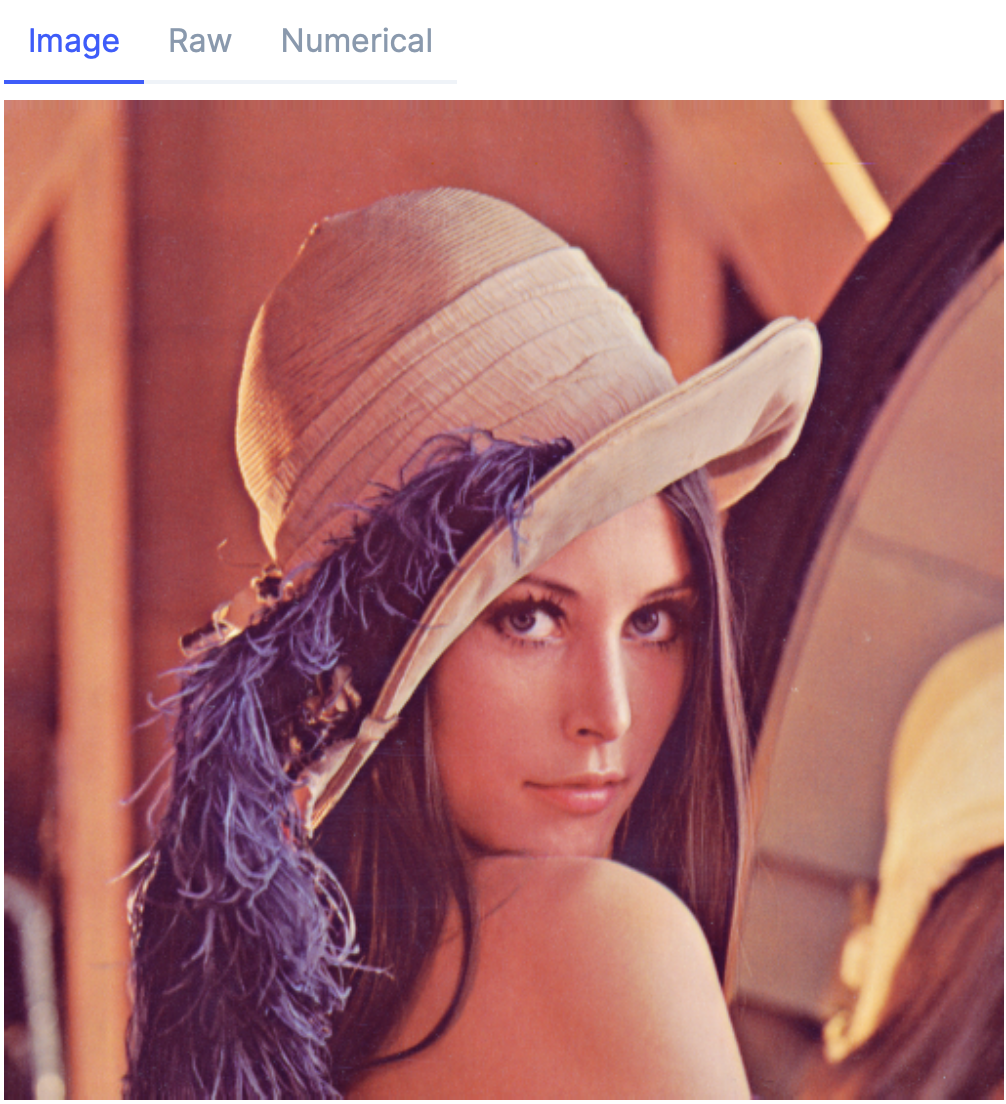
\includegraphics[scale=0.5]{ja/f3.png}
\end{center}
\caption{未処理の元の画像}
\end{figure}

次に、コマンド ラインで \textbf{iex -S mix} コマンドを使用して,Broadway パイプラインを開始する.パイプラインは連続しているため,図 4.2 に示すように最終出力のみが表示される.

\begin{figure}[H]
\vspace{5cm}
\begin{center}
\hspace{-8cm}
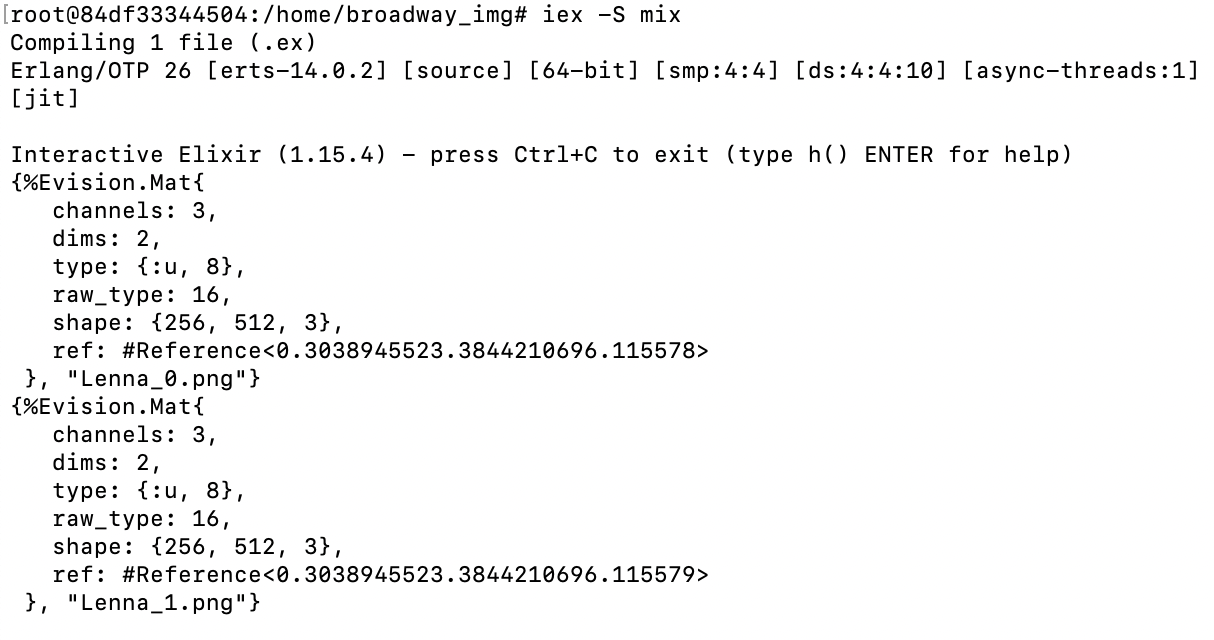
\includegraphics[scale=0.5]{ja/f9.png}
\end{center}
\caption{Broadway パイプライン最終出力}
\end{figure}

図 4.2 は,処理した画像の内容と画像名を示している.コマンドラインでは,リストを使用して処理された画像を表示する.
パイプラインを閉じると,図4.3に示すように,処理された画像ファイルがフォルダーの下に表示される.

\begin{figure}[H]
%\vspace{8cm}
\begin{center}
\hspace{-8cm}
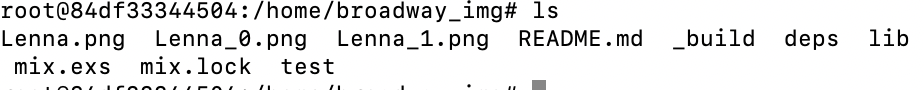
\includegraphics[scale=0.5]{ja/f8.png}
\end{center}
\caption{出力画像ファイル}
\end{figure}

パイプラインでのバッチ処理後,図 4.3 から,ファイルに Lenna\_0 と Lenna\_1 の 2 つの画像ファイルが含まれている.同じ方法を使用して両方の画像を別々に表示する.

\begin{figure}[H]
\vspace{6cm}
\begin{center}
\hspace{-8cm}
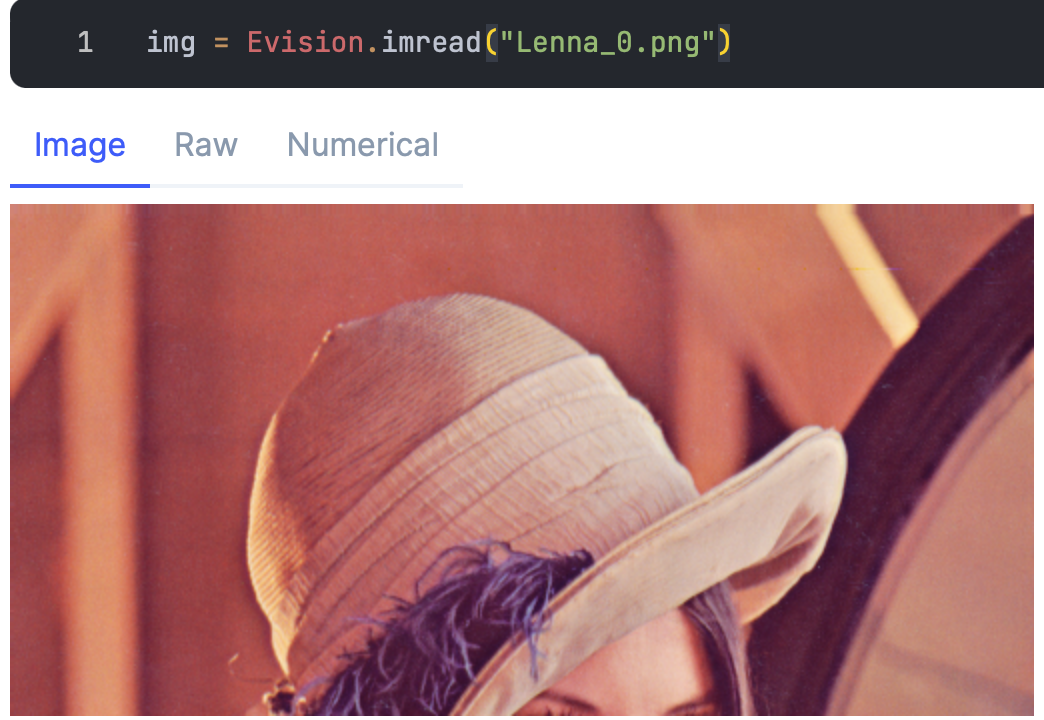
\includegraphics[scale=0.5]{ja/f4.png}
\end{center}
\caption{Lenna\_0}
\end{figure}

\begin{figure}[H]
\vspace{5cm}
\begin{center}
\hspace{-8cm}
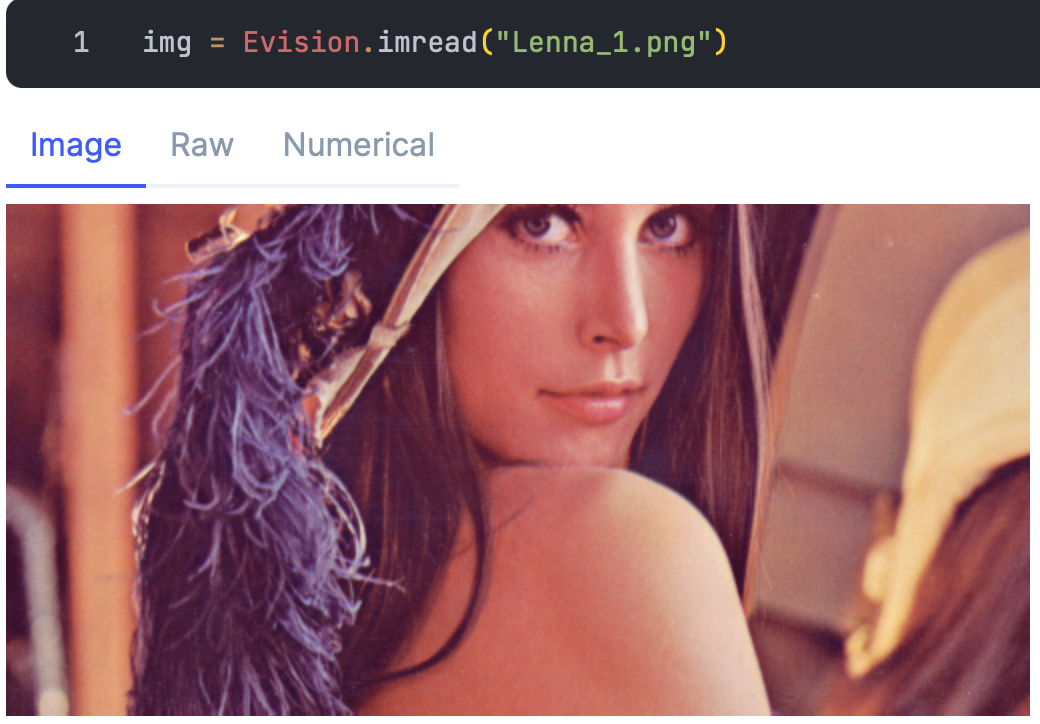
\includegraphics[scale=0.5]{ja/f5.png}
\end{center}
\caption{Lenna\_1}
\end{figure}

パイプライン分割後の画像は図4.4と4.5に示す.

図4.6と4.7に示す.分割後画像はさらに二値化する.
\begin{figure}[H]
\vspace{6cm}
\begin{center}
\hspace{-8cm}
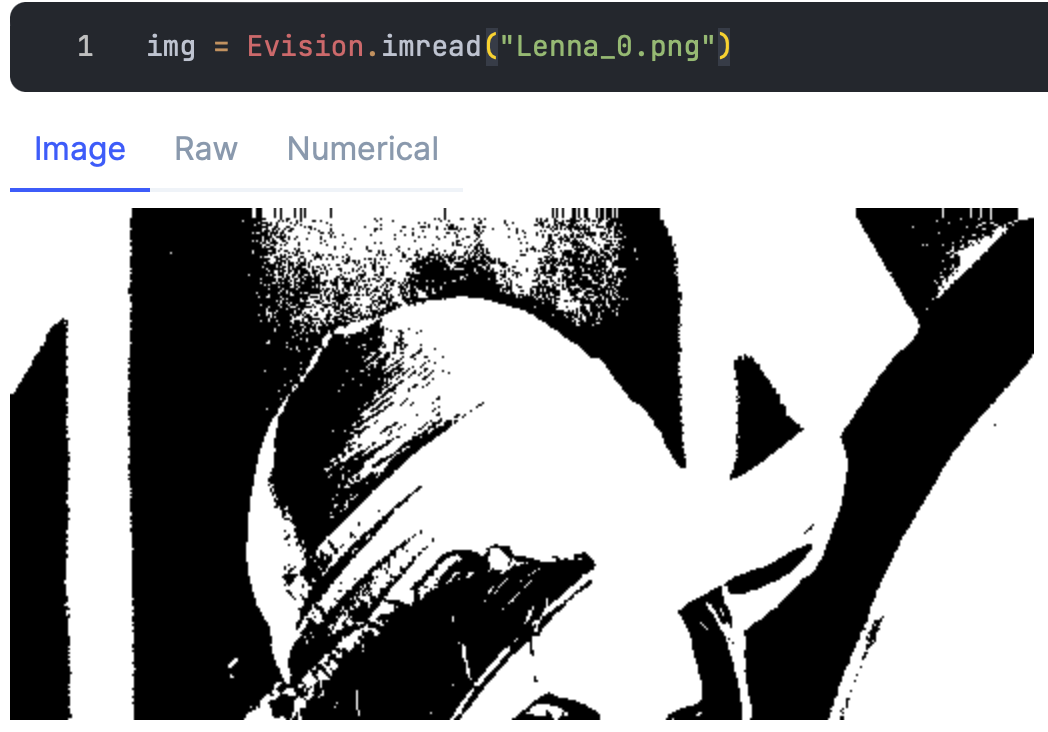
\includegraphics[scale=0.5]{ja/f6.png}
\end{center}
\caption{二値化したLenna\_0}
\end{figure}

\begin{figure}[H]
\vspace{5cm}
\begin{center}
\hspace{-8cm}
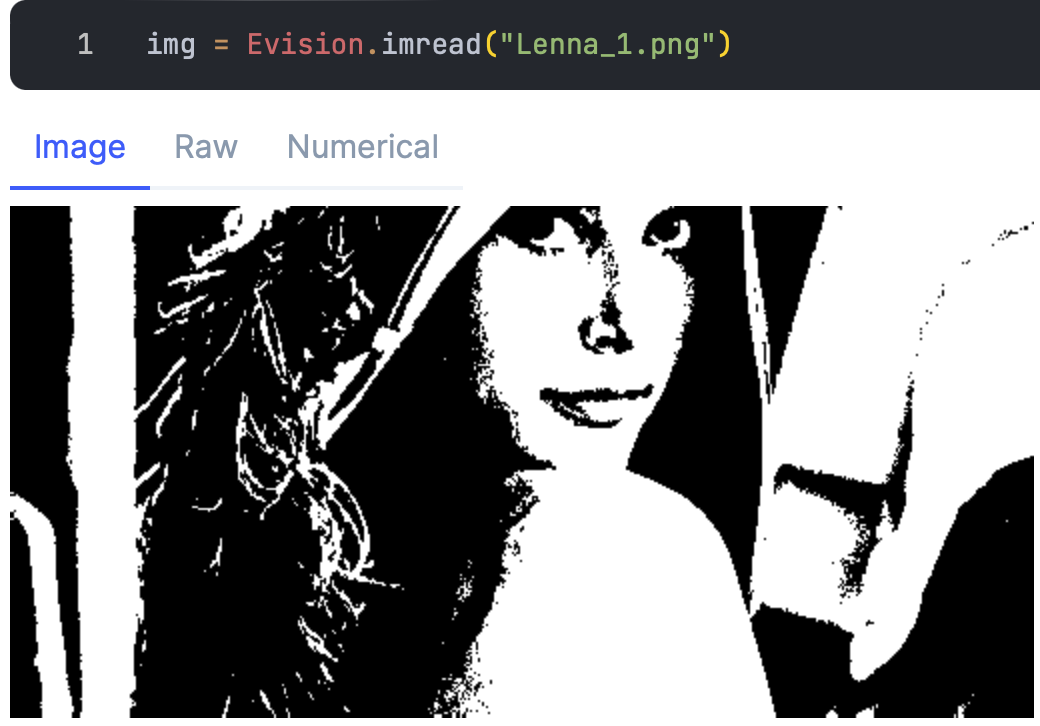
\includegraphics[scale=0.5]{ja/f7.png}
\end{center}
\caption{二値化したLenna\_1}
\end{figure}

上記の実験により,実際に Broadway のデータ取り込みとデータ処理機能を画像処理パイプラインとして活用することとが確認できた.

\subsection{Broadwayパイプラインにおける対処害機能1の評価} 
Broadway パイプラインは連続的で中断できないため,GenServerを使用してsupervisorのフォールト トレランス メカニズムを実験する.

:pop と :push を使用して,データの書き込みと読み取りをシミュレートする.:pop と :pushの定義は以下の通り.

def handle\_call(:pop, \_from, []) do

    \{:reply, :empty, []\}
    
  end

  def handle\_cast(\{:push, element\}, state) do
  
    \{:noreply, [element | state]\}
    
  end

プロセスの異常シャットダウンのロジックをシミュレートするために abort\_soft() を定義する.abort\_soft() の定義は以下の通り.

  def handle\_cast(:abort\_soft, \_state) do
  
    exit({:shutdown, :abort_soft})
    
  end

:abort\_soft メッセージが AbortNif プロセスに送信した後,メッセージは handle\_cast/2 関数によってキャプチャされ,プロセス終了処理ロジックがトリガーされる.
:abort\_soft メッセージを受信すると,exit/1 関数が呼び出され,ソフト終了信号 \{:shutdown, :abort\_soft\} が現在のプロセスに送信される.これにより,GenServerは終了信号を受信した後にプロセスを終了する.

次に,Supervisorを使用して,異常終了したプロセスを再起動できるかどうかをテストする.
Supervisorの構成は以下のとおり.

defmodule AbortNif.Application do

  \# See https://hexdocs.pm/elixir/Application.html
  
  \# for more information on OTP Applications
  
  @moduledoc false

  use Application

  @impl true
  
  def start(\_type, \_args) do
  
    children = [
    
        AbortNif

      \# Starts a worker by calling: 
      
      AbortNif.Worker.start\_link(arg)
      
      \# {AbortNif.Worker, arg}
      
    ]

    \# See https://hexdocs.pm/elixir/Supervisor.html
    
    \# for other strategies and supported options
    
    opts = [
    
    strategy: :one\_for\_one, name: 
    
    AbortNif.Supervisor
    
    ]
    
    Supervisor.start\_link(children, opts)
    
  end
  
end

実験結果を図4.8に示す.

\begin{figure}[H]
\vspace{3cm}
\begin{center}
\hspace{-8cm}
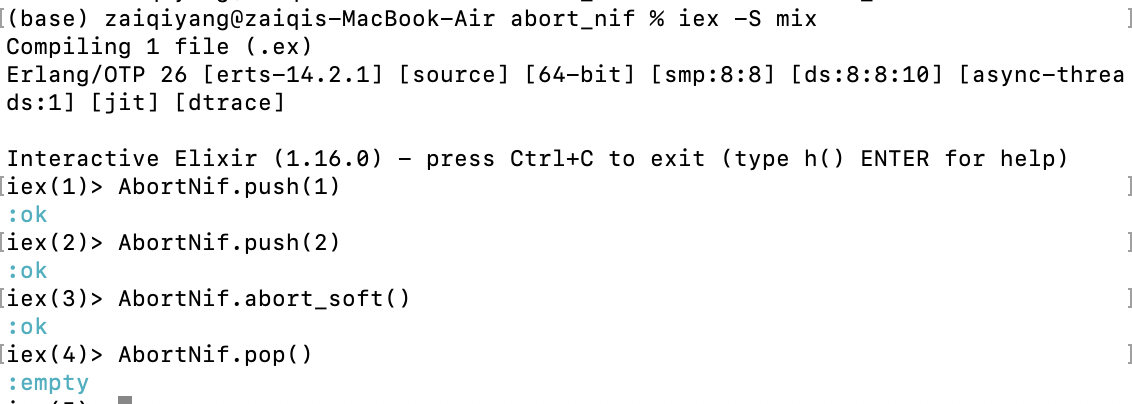
\includegraphics[scale=0.5]{ja/f11.png}
\end{center}
\caption{プロセスの異常シャットダウン}
\end{figure}

図 4.8 から,プロセスが終了した後Supervisorの監視の下でプロセスが再開され,同時に書き込まれたデータがクリアされることがわかる.

それから, Benchee を使用して, 実際にメモリ不足などによる異常終了が発生した場合, 回復速度をテストを行う.

結果を表4.1に示す.

\begin{table}[h]
  \centering
  
  \begin{tabular}{|c|c|c|c|c|c|c|c|}
    \hline
    Name & IPS & Average & Deviation & median & 99th\% \\
    \hline
Supervisor & 3.51 M  & 284.79 ns & ±6400.68\% & 250ns & 375 ns  \\
    \hline

  \end{tabular}
  \caption{supervisorの回復速度}
\end{table}


\subsection{Broadwayパイプラインにおける対処害機能2の評価}
まず,Broadwayで書かれた中止関数を呼び出す.マルチノード フォールト トレランス メカニズムを使用しない場合の結果を図 4.9 に示す.Erlang VM 全体がシャットダウンした.

\begin{figure}[H]
\vspace{1cm}
\begin{center}
\hspace{-12cm}
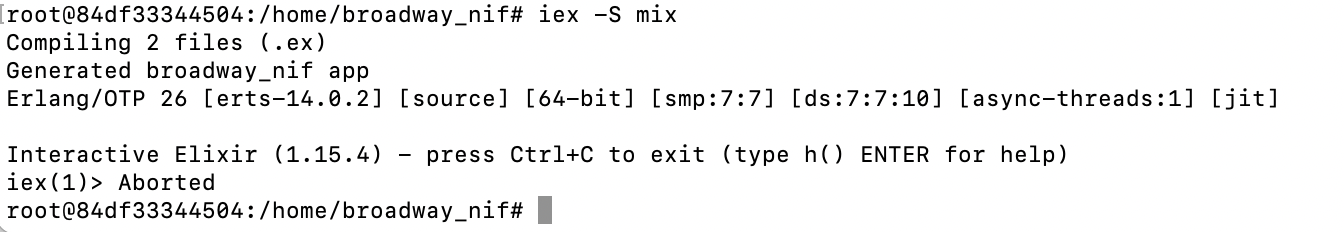
\includegraphics[scale=0.7]{ja/f10.png}
\end{center}
\caption{マルチノード フォールト トレランス 未使用}
\end{figure}

次に,Broadway パイプラインでマルチノード フォールト トレランス メカニズムを実行し,第 3 章で記述した abort\_NIf 関数を子ノードに送信する.

それから,Erlang VM が異常終了するかどうかを監視する.実験結果を図 4.10と4.11 に示す.

\begin{figure}[H]
\vspace{8cm}
\begin{center}
\hspace{-8cm}
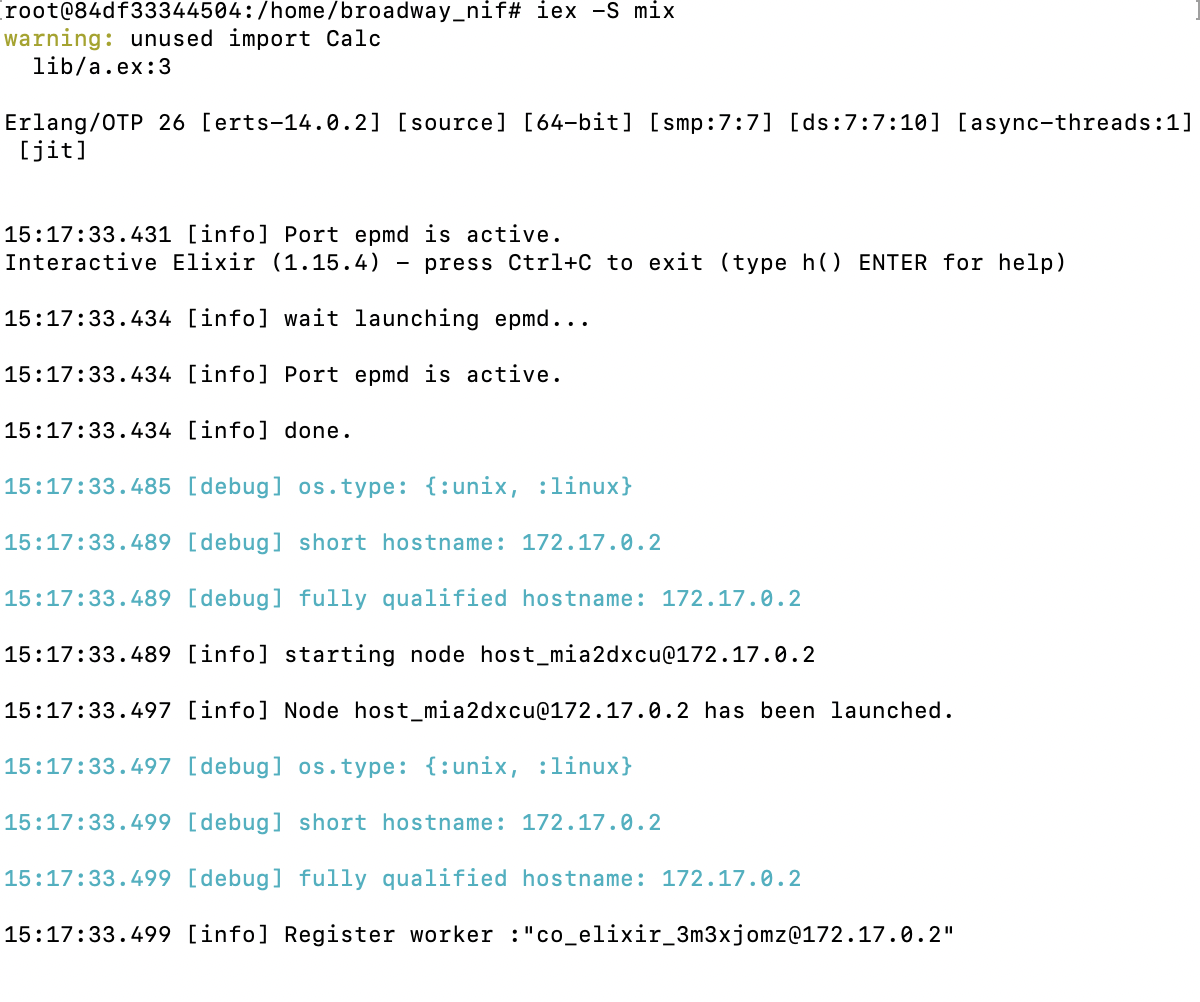
\includegraphics[scale=0.5]{ja/f12.png}
\end{center}
\caption{マルチノード フォールト トレランス 使用後1}
\end{figure}

図 4.10 から、Erlang VM がクラッシュすることなく host\_mia2dxcu@172.17.0.2 ノードと co\_elixir\_3m3xjomz@172.17.0.2 を生成した.

\begin{figure}[H]
\vspace{4cm}
\begin{center}
\hspace{-8cm}
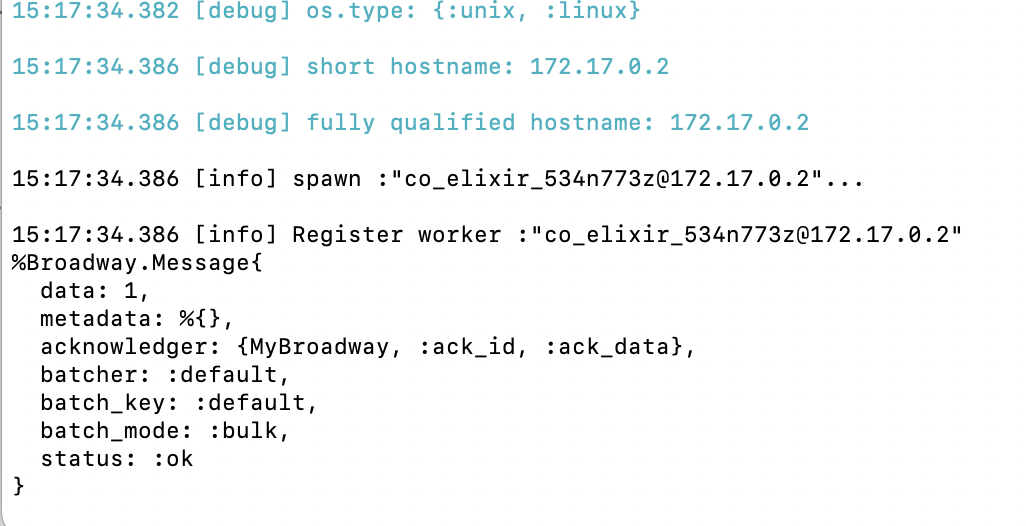
\includegraphics[scale=0.5]{ja/f13.png}
\end{center}
\caption{マルチノード フォールト トレランス 使用後2}
\end{figure}

図 4.11 からわかるように,Erlang VM はクラッシュされておらず,Broadway パイプライン内のデータは完全にコマンド ラインに出力されている.




\chapter{まとめと将来課題}
\section{まとめ}
本研究では,Elixir のライブラリ関数であるNodeによるマルチノードのフォールトトレランスとBroadwayによるSupervisorの耐障害性を活用したパイプラインを提案した.

まず,実験1でパイプラインを使用して,画像を読み取り,グレースケール画像に変換した.次に,Evision.threshold/3 を使用してグレースケールイメージをしきい値処理して,バイナリイメージを取得した.最後に,Nx.to\_batched/2 を使用してイメージを分割し,Enum.zip/2 を使用して分割イメージと以前に生成されたファイル名をペアにしてから,各画像は対応するファイルとして保存された.実験1により画像のバッチ処理を実現できた.

また, 実験2で abort\_soft()関数が異常終了し, 再起動されたから, supervisorのフォールト トレランス 機能を確認した. 同時に, Bencheeでabort\_soft()関数の平均復帰時間は284.79 nsのデータを取得した. 

実験2によりSupervisor を用いることで画像処理プロセスが何らかの理由により障害が発生した場合におけるタスクの高速な復帰を実現できる結論が得られた. 

さらに,実験3でSpawnCoElixirを実装なしの Broadwayパイプラインと実装された Broadway パイプラインを比較して, 2 つのパイプラインの最初の段階で第 3 章で記述した abort\_NIF 関数を呼び出した. 実験結果は, SpawnCoElixirを実装されないBroadwayパイプラインとErlang VMが同時にクラッシュした. SpawnCoElixirを実装された Broadwayパイプラインはクラッシュしなっかた, そしてプロデューサー データは消費するワーカーに正常に渡された.

実験3によりElixirのライブラリ関数であるSpawnCoElixirの動作における親と子のノード間のメッセージ通信を介して,クラッシュの原因となる NIF 関数は子ノードで呼び出されて,子のノードがクラッシュした後でも,親ノードが影響を受けない結論が得られた.

Broadway フレームワークを導入し,耐障害性と並列性の向上と組み合わせることで,画像バッチ処理の効率と信頼性が向上した.改良されたプロセスにより,大規模な画像処理タスクへの適応性が高まり,さまざまな異常事態への対処が向上する。

\section{将来課題}
今後の課題として,エラー処理の改善など,耐障害性の改善を引き続き強化する.例えば,ノード構成で最大再試行回数を設定して,ノードがメッセージを処理しているときにエラーが発生した場合,後で処理を再試行できるようにする.そして複数のステップを伴う処理のために,エラーが発生したときに以前の状態に安全にロールバックしてデータの不整合を回避できるようにする色々なメカニズムが導入することを考える.
\chapter*{謝辞}
この論文の執筆にあたり,多くの方々にご支援いただきました. まず,指導教員である山崎進先生に深く感謝申し上げます. 先生の専門的な知識と的確なアドバイスは,私の研究を大きく前進させる助けとなりました. また,多忙な中でも丁寧なご指導を賜り,心より感謝申し上げます. 

私の家族や友人にも深い感謝を捧げます. 彼らの理解と励ましは,私が研究に専念できる大きな支えとなりました. 

最後に, これまで私を支えてくださったすべての方々に心からの感謝を申し上げます. 皆様のおかげで,この論文を完成させることができました. 

本研究の一部は,北九州産業学術推進機構(FAIS) 旭興産グループ研究支援プログラムの支援を受けた.
\addcontentsline{toc}{chapter}{謝辞}



% 参考文献(References)
\newpage
\addcontentsline{toc}{chapter}{参考文献}
\renewcommand{\bibname}{参考文献}

%% 参考文献に bibtex を使う場合
%\bibliographystyle{junsrt}
%\bibliography{hoge}

%% 参考文献を直接ファイルに含めて書く場合
\begin{thebibliography}{99}

% e.g.)
\bibitem{A}
Tom B. Brown, Benjamin Mann et al. 2020. Language models are few-shot learners. In Proceedings of the 34th International Conference on Neural Information Processing Systems (NIPS'20). Curran Associates Inc. Red Hook, NY, USA, Article 159, 1877--1901.

\bibitem{B}
Jean Bacon 1996. Concurrent Systems: An Integrated Approach to Operating Systems, Distributed Systems and Database. Addison-Wesley. pp.265--276.

\bibitem{C}
山崎進,森正和,上野嘉大,高瀬英希: Hastega: Elixir プログラミングにおける超並列化を実現するための GPGPU 活用手法,情報処理学会第120回プログラミング研究会, Vol. 2018,No. 2,pp. 8,2018.
\bibitem{D}
Broadway: Build concurrent and multi-stage data ingestion and data processing pipelines with Elixir \url{https://github.com/dashbitco/broadway} (2023.10.2).

\bibitem{E}
Susumu Yamazaki: Robust, Distributed, and Parallel Processing for Enormous Images \url{https://www.youtube.com/watch?v=RkMzCQm-Ws4t=1087s} (2023.11.12).
\bibitem{F}
Hsueh, M.-C., Tsai, T.K. and Iyer, R.K.: Fault Injection Techniques and Tools, IEEE Computer, Vol.30, No.4, pp.75--82 (1997).
\bibitem{G}
The Elixir Team: Elixir is a dynamic, functional language designed for building scalable and maintainable applications \url{https://elixir-lang.org}. (online), \url{https://github.com/elixir-lang/elixir} (2023.07.20).
\bibitem{H}
The Elixir Team: Functions related to VM nodes. Retrieved June 20, 2023 from \url{https://hexdocs.pm/elixir/1.16.0-rc.0/Node.html}
\bibitem{I}
Alexandre Jorge Barbosa Rodrigues and Viktória Fördős. 2018. To- wards Secure Erlang Systems. In Proceedings of the 17th ACM SIGPLAN International Workshop on Erlang (Erlang 2018). ACM, New York, NY, USA, 67--70. \url{https://doi.org/10.1145/3239332.3242768}
\bibitem{J}
Ericsson AB: Erlang Kernel Reference Manual Version 6.4, net kernel:monitor nodes. Retrieved June 20, 2023 from \url{http://erlang.org/doc/man/net_kernel.html}.

\bibitem{M}
The Elixir Team: GenServer: A behaviour module for implementing the server of a client-server. \url{https://hexdocs.pm/elixir/GenServer.html}  

\bibitem{N}
SpawnCoElixir: spawns cooperative Elixir nodes that are supervised. \url{https://hexdocs.pm/spawn_co_elixir/SpawnCoElixir.html} (2024.1.13).

\bibitem{O}
Benchee: Library for easy and nice (micro) benchmarking in Elixir.
\url{https://hexdocs.pm/benchee/Benchee.html} (2024.1.13).

\chapter*{付録}


\end{thebibliography}

\end{document}
